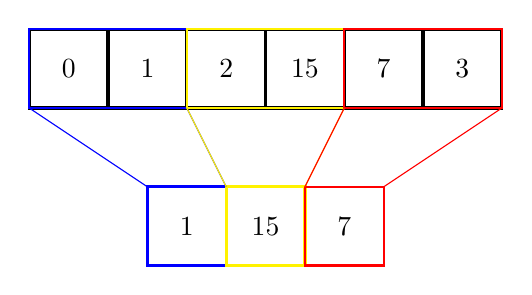
\begin{tikzpicture}[
neuron/.style={circle, draw=black, very thick, minimum size=1cm, transform shape},
dot/.style={circle, draw=black, fill=black, minimum size=0.1cm, inner sep=0pt, transform shape},
note/.style={circle, draw=black, minimum size=0pt, inner sep=0pt, transform shape},
]
%Input
\draw[black, very thick] (0,  0) rectangle (1, -1) node[pos=0.5] {0};
\draw[black, very thick] (1,  0) rectangle (2, -1) node[pos=0.5] {1};
\draw[black, very thick] (2,  0) rectangle (3, -1) node[pos=0.5] {2};
\draw[black, very thick] (3,  0) rectangle (4, -1) node[pos=0.5] {15};
\draw[black, very thick] (4,  0) rectangle (5, -1) node[pos=0.5] {7};
\draw[black, very thick] (5,  0) rectangle (6, -1) node[pos=0.5] {3};

%Filter boxes layer 1
\draw[blue, thick] (0,  0) rectangle (2, -1);
\draw[yellow, thick] (2, 0) rectangle (4, -1);
\draw[red, thick] (4, 0) rectangle (6, -1);

%Layer 2
\draw[blue, very thick] (1.5, -2) rectangle (2.5, -3) node[pos=0.5, black] {1};
\draw[yellow, very thick] (2.5, -2) rectangle (3.5, -3) node[pos=0.5, black] {15};
\draw[red, thick] (3.5, -2) rectangle (4.5, -3) node[pos=0.5, black] {7};

%Connections layer 1 -- layer 2
\draw[blue] (0, -1) -- (1.5, -2);
\draw[blue] (2, -1) -- (2.5, -2);
\draw[yellow] (2, -1) -- (2.5, -2);
\draw[yellow] (4, -1) -- (3.5, -2);
\draw[red] (4, -1) -- (3.5, -2);
\draw[red] (6, -1) -- (4.5, -2);
\end{tikzpicture}